% vim: set spell spelllang=en tw=100 et sw=4 sts=4 foldmethod=marker foldmarker={{{,}}} :

\documentclass[aspectratio=169,compress,10pt]{beamer}

\usepackage{tikz}
\usepackage{xcolor}
\usepackage{complexity}
\usepackage{hyperref}
\usepackage{microtype}
\usepackage{amsmath}                   % \operatorname
\usepackage{amsfonts}                  % \mathcal
\usepackage{amssymb}                   % \nexists
\usepackage[vlined]{algorithm2e} % algorithms
\usepackage{centernot}
\usepackage{listings}
\usepackage{csquotes}
\usepackage{fancyvrb}
\usepackage{bussproofs}
\usepackage{multicol}
\usepackage{booktabs}
\usepackage{mathtools}
\usepackage{pifont}
\usepackage{marvosym}
\usepackage{cancel}

\usefonttheme{professionalfonts}

\usetikzlibrary{shapes, arrows, shadows, calc, positioning, fit}
\usetikzlibrary{decorations.pathreplacing, decorations.pathmorphing, shapes.misc}
\usetikzlibrary{tikzmark, backgrounds}
\usetikzlibrary{trees, overlay-beamer-styles}

\tikzset{processarrow/.style={->, very thick, decorate, decoration={snake, post length=0.5mm}}}
\tikzset{brace/.style={decorate, decoration={brace}, very thick}}

\definecolor{uofguniversityblue}{rgb}{0, 0.219608, 0.396078}
\definecolor{uofgheather}{rgb}{0.356863, 0.32549, 0.490196}
\definecolor{uofgaquamarine}{rgb}{0.603922, 0.72549, 0.678431}
\definecolor{uofgslate}{rgb}{0.309804, 0.34902, 0.380392}
\definecolor{uofgrose}{rgb}{0.823529, 0.470588, 0.709804}
\definecolor{uofgmocha}{rgb}{0.709804, 0.564706, 0.47451}
\definecolor{uofgsandstone}{rgb}{0.321569, 0.278431, 0.231373}
\definecolor{uofgforest}{rgb}{0, 0.2, 0.129412}
\definecolor{uofglawn}{rgb}{0.517647, 0.741176, 0}
\definecolor{uofgcobalt}{rgb}{0, 0.615686, 0.92549}
\definecolor{uofgturquoise}{rgb}{0, 0.709804, 0.819608}
\definecolor{uofgsunshine}{rgb}{1.0, 0.862745, 0.211765}
\definecolor{uofgpumpkin}{rgb}{1.0, 0.72549, 0.282353}
\definecolor{uofgthistle}{rgb}{0.584314, 0.070588, 0.447059}
\definecolor{uofgrust}{rgb}{0.603922, 0.227451, 0.023529}
\definecolor{uofgburgundy}{rgb}{0.490196, 0.133333, 0.223529}
\definecolor{uofgpillarbox}{rgb}{0.701961, 0.047059, 0}
\definecolor{uofglavendar}{rgb}{0.356863, 0.301961, 0.580392}

% {{{ theme things
\useoutertheme[footline=authortitle]{miniframes}
\useinnertheme{rectangles}

\setbeamerfont{block title}{size={}}
\setbeamerfont{title}{size=\large,series=\bfseries}
\setbeamerfont{section title}{size=\large,series=\mdseries}
\setbeamerfont{author}{size=\normalsize,series=\mdseries}
\setbeamercolor*{structure}{fg=uofguniversityblue}
\setbeamercolor*{palette primary}{use=structure,fg=black,bg=white}
\setbeamercolor*{palette secondary}{use=structure,fg=white,bg=uofgcobalt}
\setbeamercolor*{palette tertiary}{use=structure,fg=white,bg=uofguniversityblue}
\setbeamercolor*{palette quaternary}{fg=white,bg=black}
\setbeamercolor{block body}{bg=structure!10}
\setbeamercolor{block title}{bg=structure,fg=white}
\setbeamertemplate{blocks}[rounded]
\setbeamercolor*{titlelike}{parent=palette primary}

\beamertemplatenavigationsymbolsempty

\setbeamertemplate{title page}
{
    \begin{tikzpicture}[remember picture, overlay]
        \node at (current page.north west) {
            \begin{tikzpicture}[remember picture, overlay]
                \fill [fill=uofguniversityblue, anchor=north west] (0, 0) rectangle (\paperwidth, -2.6cm);
            \end{tikzpicture}
        };

        \node (logo) [anchor=north east, shift={(-0.8cm,-0.2cm)}] at (current page.north east) {
            
\includegraphics[keepaspectratio=true,scale=0.5]{../../images/UoG_keyline.pdf}
        };

        \node (logo2) [anchor=north, below=0.2cm of logo.south] {
            
\includegraphics[keepaspectratio=true,scale=0.1]{../../images/RAEngWhite.pdf}
        };

        \coordinate (logos) at ($(logo.south)!0.5!(logo2.north)$);

        \node [anchor=west, xshift=0.8cm] at (current page.west |- logos) {
            \begin{minipage}{0.65\paperwidth}\raggedright
                {\usebeamerfont{title}\usebeamercolor[white]{}\inserttitle}\\[0.1cm]
                {\usebeamerfont{author}\usebeamercolor[white]{}\insertauthor}\\[0.2cm]
                {\usebeamerfont{author}\usebeamercolor[white]{}\scriptsize In collaboration with Matthew
                McIlree; Emir Demirovi\'c and Konstantin
                                Sidorov (TU Delft);\\[-0.1cm]and Jakob Nordstr\"om and Andy Oertel (Lund
                                University / University of Copenhagen)}
            \end{minipage}
        };
    \end{tikzpicture}
}

\setbeamertemplate{section page}
{
    \begin{centering}
        \begin{beamercolorbox}[sep=12pt,center]{part title}
            \usebeamerfont{section title}\insertsection\par
        \end{beamercolorbox}
    \end{centering}
}

\newcommand{\frameofframes}{/}
\newcommand{\setframeofframes}[1]{\renewcommand{\frameofframes}{#1}}

\makeatletter
\setbeamertemplate{footline}
{%
    \begin{beamercolorbox}[colsep=1.5pt]{upper separation line foot}
    \end{beamercolorbox}
    \begin{beamercolorbox}[ht=2.5ex,dp=1.125ex,%
        leftskip=.3cm,rightskip=.3cm plus1fil]{author in head/foot}%
        \leavevmode{\usebeamerfont{author in head/foot}\insertshortauthor}%
        \hfill%
        {\usebeamerfont{institute in head/foot}\usebeamercolor[fg]{institute in head/foot}\insertshortinstitute}%
    \end{beamercolorbox}%
    \begin{beamercolorbox}[ht=2.5ex,dp=1.125ex,%
        leftskip=.3cm,rightskip=.3cm plus1fil]{title in head/foot}%
        {\usebeamerfont{title in head/foot}\insertshorttitle}%
        \hfill%
        {\usebeamerfont{frame number}\usebeamercolor[fg]{frame number}\insertframenumber~\frameofframes~\inserttotalframenumber}
    \end{beamercolorbox}%
    \begin{beamercolorbox}[colsep=1.5pt]{lower separation line foot}
    \end{beamercolorbox}
}

\makeatletter
\setbeamertemplate{mini frame}
{%
  \begin{pgfpicture}{0pt}{0pt}{.04cm}{.04cm}
    \pgfpathcircle{\pgfpoint{0.04cm}{0.04cm}}{0.04cm}
    \pgfusepath{fill,stroke}
  \end{pgfpicture}%
}
\setbeamertemplate{mini frame in current subsection}
{%
  \begin{pgfpicture}{0pt}{0pt}{.04cm}{.04cm}
    \pgfpathcircle{\pgfpoint{0.04cm}{0.04cm}}{0.04cm}
    \pgfsetfillcolor{section in head/foot.bg}
    \pgfusepath{fill,stroke}
  \end{pgfpicture}%
}

\setbeamersize{mini frame size=0.10cm, mini frame offset=0.06cm}
\makeatother

\makeatletter
\newenvironment{nearlyplainframe}[2][]{
    \def\beamer@entrycode{\vspace*{-\headheight}\vspace*{3pt}}
    \setbeamertemplate{headline}
    {%
        \begin{beamercolorbox}[colsep=1.5pt]{upper separation line head}
        \end{beamercolorbox}
        \begin{beamercolorbox}[ht=0.5ex,dp=0.125ex,%
            leftskip=.3cm,rightskip=.3cm plus1fil]{title in head/foot}%
        \end{beamercolorbox}%
        \begin{beamercolorbox}[ht=0.5ex,dp=0.125ex,%
            leftskip=.3cm,rightskip=.3cm plus1fil]{author in head/foot}%
        \end{beamercolorbox}%
        \begin{beamercolorbox}[colsep=1.5pt]{lower separation line head}
        \end{beamercolorbox}
        \vspace*{\headheight}
    }

    \setbeamertemplate{footline}
    {%
        \begin{beamercolorbox}[colsep=1.5pt]{upper separation line foot}
        \end{beamercolorbox}
        \begin{beamercolorbox}[ht=0.5ex,dp=0.125ex,%
            leftskip=.3cm,rightskip=.3cm plus1fil]{author in head/foot}%
        \end{beamercolorbox}%
        \begin{beamercolorbox}[ht=0.5ex,dp=0.125ex,%
            leftskip=.3cm,rightskip=.3cm plus1fil]{title in head/foot}%
        \end{beamercolorbox}%
        \begin{beamercolorbox}[colsep=1.5pt]{lower separation line foot}
        \end{beamercolorbox}
    }

    \begin{frame}[#1]{#2}
    }{
    \end{frame}
}
\makeatother

% }}}

\addtolength{\jot}{5pt}

\tikzstyle{state} = [inner sep=1pt]
\tikzstyle{infeasible} = [color=uofgpillarbox]
\tikzstyle{dominated} = [color=uofgcobalt]
\tikzstyle{backwards} = [color=uofgpumpkin]
\tikzstyle{accept} = [solid, thick]
\tikzstyle{reject} = [dotted, thick]
\tikzstyle{domination} = [dashed, thick, ->, color=uofgcobalt]

\author{Ciaran McCreesh}
\title{Proof Logging for Dynamic Programming Algorithms}

\begin{document}

{
    \usebackgroundtemplate{
        \tikz[overlay, remember picture]
        \node[at=(current page.south), anchor=south, inner sep=0pt, yshift=-1.4cm]{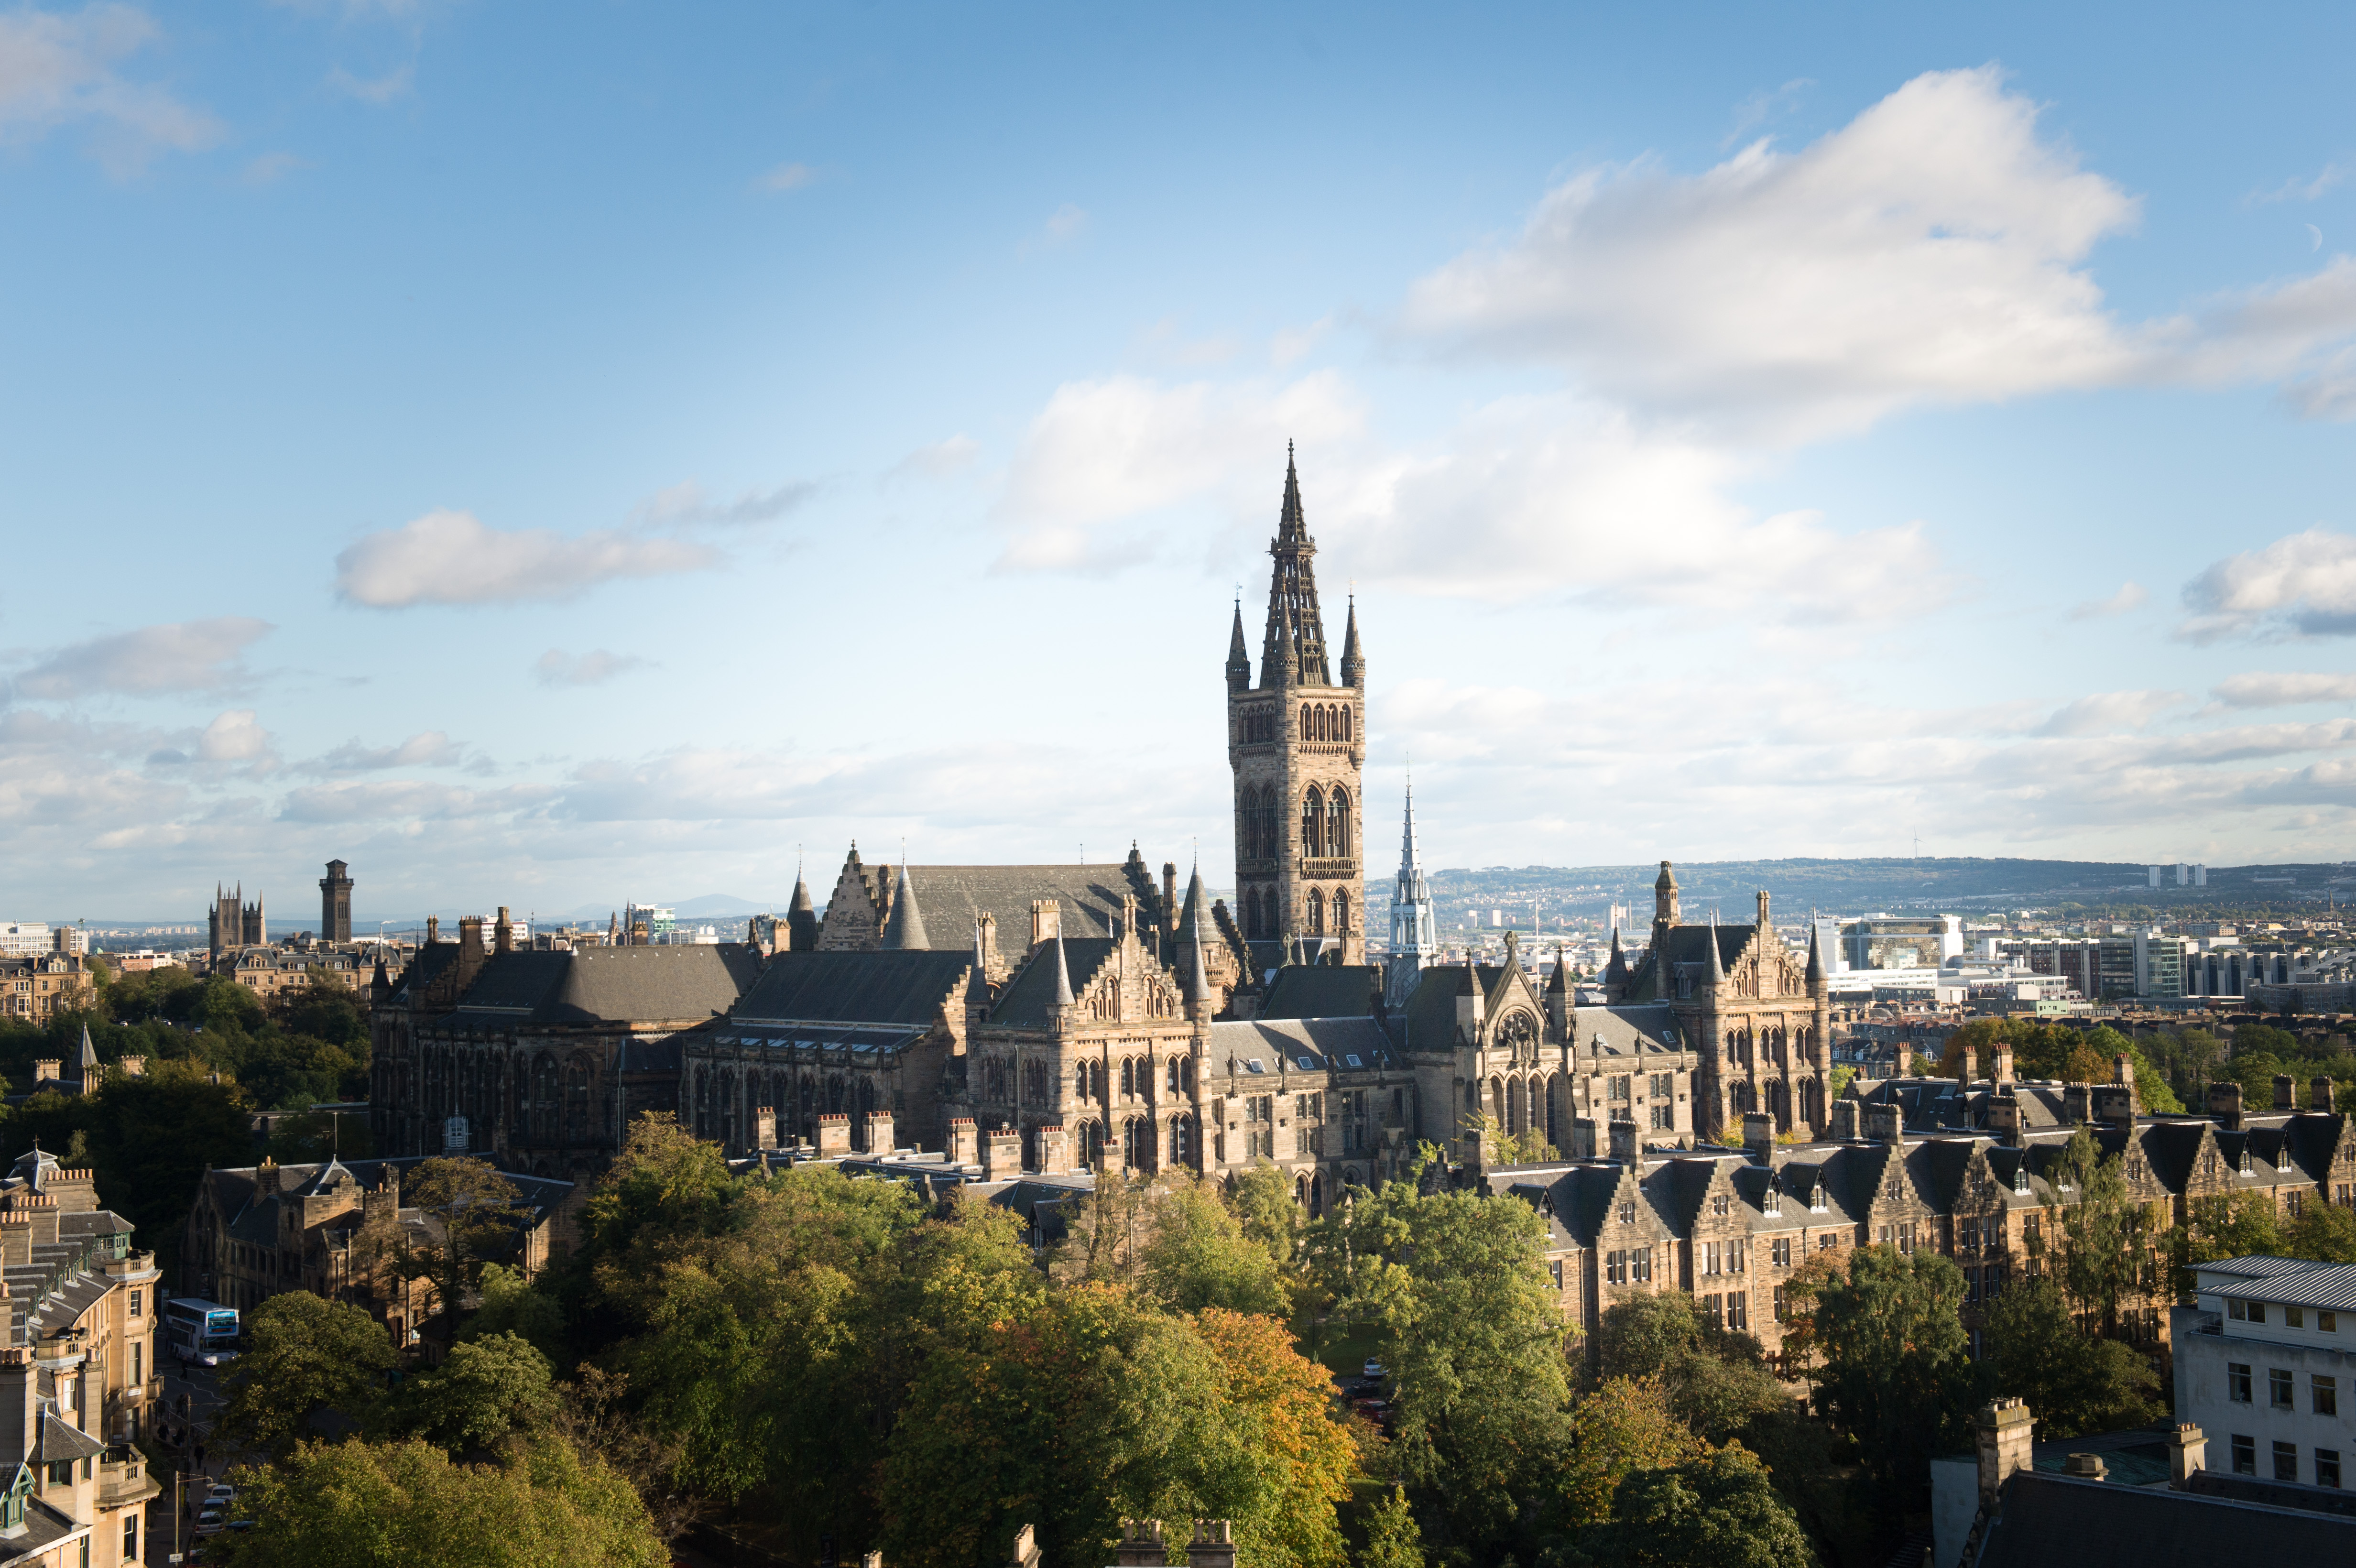
\includegraphics[keepaspectratio=true, width=\paperwidth]{../../images/background.jpg}};
    }
    \begin{frame}[plain,noframenumbering]
        \titlepage
    \end{frame}
}

\section{Knapsack}

\begin{frame}{Knapsack Problems}
    \begin{align*}
        &x_i \in \{0, 1\} && \text{whether or not we take item $i$}\\
        &\sum_i \boldsymbol{w}_i x_i \le W && \text{total weight of items taken not too heavy}\\
        &\operatorname{maximise} \sum_i \boldsymbol{p}_i x_i && \text{yay capitalism}
    \end{align*}

    For our running example,
    \begin{align*}
        \boldsymbol{w} &= [2, 5, 2, 3, 2, 3] \text{~and}\\
        \boldsymbol{p} &= [2, 4, 2, 5, 4, 3] \text{~with}\\
        W &\le 7
    \end{align*}

\end{frame}

\begin{frame}{Dynamic Programming for Knapsack}
    To decide whether we're taking the $i$th item, with $w$ weight available to spend,
    \begin{align*}
        & P(i, w) = \operatorname{max}(\\
        &     \qquad P(i - 1, w),\\
        &     \qquad P(i - 1, w - \boldsymbol{w}_i) + \boldsymbol{p}_i \text{~if~} \boldsymbol{w}_i \le w \\
        & ) \\ \medskip
        & P(0, w) = 0
    \end{align*}
\end{frame}

\begin{frame}{Sparse Dynamic Programming}
    Key ideas:
    \begin{itemize}
        \item ``Maximum'' selects between partial sums on the same items with the same
            combined weights but different profits.
        \item Don't calculate the same state more than once.
        \item Only calculate partial sums of weights and profits that can actually be
            achieved.
    \end{itemize}
    \bigskip
    Algorithmic details matter a lot for performance but end up being more or less the same for proof logging.
\end{frame}

\begin{frame}{Merging More States}
    The ``maximum'' means, if we could reach states \begin{equation*}
        \sum_{i=1}^{\ell} \boldsymbol{w}_i = w \text{~and~} \sum_{i=1}^{\ell} \boldsymbol{p}_i = p
        \qquad \text{or} \qquad
        \sum_{i=1}^{\ell} \boldsymbol{w}_i = w \text{~and~} \sum_{i=1}^{\ell} \boldsymbol{p}_i = p'
    \end{equation*}
    with $p > p'$ then we only need to consider the state with profit $p$.

    \bigskip

    \uncover<2->{
    More generally, if we have two states
    \begin{equation*}
            \sum_{i=1}^{\ell} \boldsymbol{w}_i = w \text{~and~} \sum_{i=1}^{\ell} \boldsymbol{p}_i = p
            \qquad \text{or} \qquad
            \sum_{i=1}^{\ell} \boldsymbol{w}_i = w' \text{~and~} \sum_{i=1}^{\ell} \boldsymbol{p}_i = p'
    \end{equation*}
    with $p \ge p'$ and $w \le w'$ then we need only consider the former.

    \bigskip

    Whether or not this can be detected efficiently depends upon how the algorithm is implemented.}
\end{frame}

\begin{nearlyplainframe}[t]{Viewing Dynamic Programming as a Decision Diagram}
\tikzstyle{level 1}=[level distance=2.20cm, sibling distance=3.00cm]
\tikzstyle{level 2}=[level distance=2.20cm, sibling distance=2.00cm]
\tikzstyle{level 3}=[level distance=2.20cm, sibling distance=1.25cm]
\tikzstyle{level 4}=[level distance=2.20cm, sibling distance=0.75cm]
\tikzstyle{level 5}=[level distance=2.20cm, sibling distance=0.60cm]
\tikzstyle{level 6}=[level distance=2.20cm, sibling distance=0.30cm]
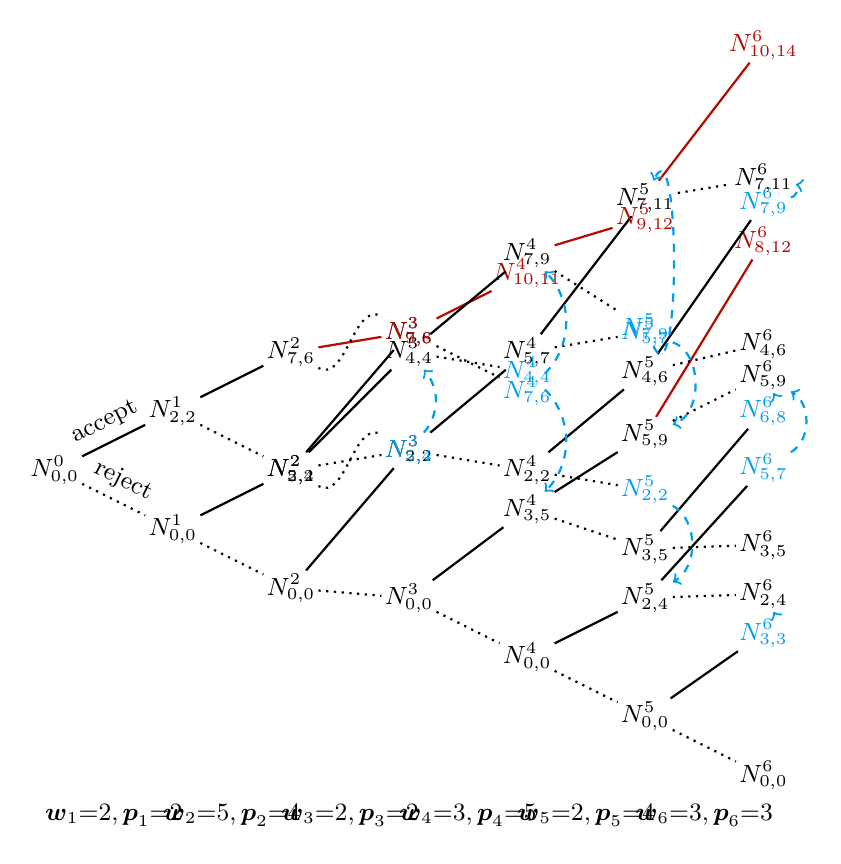
\begin{tikzpicture}[grow=right, sloped, font=\small]
    \node (N0w0p0) [state] {$N^0_{0,0}$}
    child {
        node (N1w0p0) [state] {$N^1_{0,0}$}
        child {
            node (N2w0p0) [state] {$N^2_{0,0}$}
            child {
                node (N3w0p0) [state, yshift=0.625cm] {$N^3_{0,0}$}
                child {
                    node (N4w0p0) [state] {$N^4_{0,0}$}
                    child {
                        node (N5w0p0) [state] {$N^5_{0,0}$}
                        child {
                            node (N6w0p0) [state] {$N^6_{0,0}$}
                            edge from parent [reject]
                        }
                        child {
                            node (N6w3p3) [state, dominated, yshift=0.3cm] {$N^6_{3,3}$}
                            edge from parent [accept]
                        }
                        edge from parent [reject]
                    }
                    child {
                        node (N5w2p4) [state] {$N^5_{2,4}$}
                        child {
                            node (N6w2p4) [state, yshift=0.8cm] {$N^6_{2,4}$}
                            edge from parent [reject]
                        }
                        child {
                            node (N6w5p7) [state, dominated, yshift=0.9cm] {$N^6_{5,7}$}
                            edge from parent [accept]
                        }
                        edge from parent [accept]
                    }
                    edge from parent [reject]
                }
                child {
                    node (N4w3p5) [state, yshift=0.375cm] {$N^4_{3,5}$}
                    child {
                        node (N5w3p5) [state, yshift=0.25cm] {$N^5_{3,5}$}
                        child {
                            node (N6w3p5) [state, yshift=0.8cm] {$N^6_{3,5}$}
                            edge from parent [reject]
                        }
                        child {
                            node (N6w6p8) [state, dominated, yshift=1cm] {$N^6_{6,8}$}
                            edge from parent [accept]
                        }
                        edge from parent [reject]
                    }
                    child {
                        node (N5w5p9) [state, yshift=0.2cm] {$N^5_{5,9}$}
                        child {
                            node (N6w5p9) [state, yshift=1.5cm] {$N^6_{5,9}$}
                            edge from parent [reject]
                        }
                        child {
                            node [state, infeasible, yshift=1.7cm] {$N^6_{8,12}$}
                            edge from parent [accept, infeasible]
                        }
                        edge from parent [accept]
                    }
                    edge from parent [accept]
                }
                edge from parent [reject]
            }
            child {
                node (N3w2p2) [state, yshift=1cm] {$N^3_{2,2}$}
                child {
                    node [state, yshift=0.5cm] {$N^4_{2,2}$}
                    child {
                        node (N5w2p2) [state, dominated, yshift=0.5cm] {$N^5_{2,2}$}
                        edge from parent [reject]
                    }
                    child {
                        node (N5w4p6) [state, yshift=0.5cm] {$N^5_{4,6}$}
                        child {
                            node [state, yshift=1.1cm] {$N^6_{4,6}$}
                            edge from parent [reject]
                        }
                        child {
                            node (N6w7p9) [state, dominated, yshift=1.4cm] {$N^6_{7,9}$}
                            edge from parent [accept]
                        }
                        edge from parent [accept]
                    }
                    edge from parent [reject]
                }
                child {
                    node [state, yshift=0.5cm] {$N^4_{5,7}$}
                    child {
                        node (N5w5p7) [state, dominated, yshift=1.0cm] {$N^5_{5,7}$}
                        edge from parent [reject]
                    }
                    child {
                        node (N5w7p11) [state, yshift=1.2cm] {$N^5_{7,11}$}
                        child {
                            node (N6w7p11) [state, yshift=1cm] {$N^6_{7,11}$}
                            edge from parent [reject]
                        }
                        child {
                            node [state, infeasible, yshift=1.2cm] {$N^6_{10,14}$}
                            edge from parent [accept, infeasible]
                        }
                        edge from parent [accept]
                    }
                    edge from parent [accept]
                }
                edge from parent [accept]
            }
            edge from parent [reject]
        }
        child {
            node (N2w5p5) [state] {$N^2_{5,4}$}
            child {
                node (N3w5p4) [state, dominated, yshift=1cm] {$N^3_{5,4}$}
                edge from parent [reject]
            }
            child {
                node (N3w7p6) [state, yshift=1cm] {$N^3_{7,6}$}
                child {
                    node (N4w7p6) [state, dominated] {$N^4_{7,6}$}
                    edge from parent [reject]
                }
                child {
                    node [state, infeasible] {$N^4_{10,11}$}
                    edge from parent [accept, infeasible]
                }
                edge from parent [accept]
            }
            edge from parent [accept]
        }
        edge from parent [reject] node [midway, above] { reject }
    }
    child {
        node [state] {$N^1_{2,2}$}
        child {
            node (N2w2p2) [state] {$N^2_{2,2}$}
            child {
                node (N3w4p4) [state, yshift=1.5cm] {$N^3_{4,4}$}
                child {
                    node (N4w4p4) [state, dominated, yshift=0.5cm] {$N^4_{4,4}$}
                    edge from parent [reject]
                }
                child {
                    node (N4w7p9) [state, yshift=0.5cm] {$N^4_{7,9}$}
                    child {
                        node (N5w7p9) [state, dominated, yshift=-0.2cm] {$N^5_{7,9}$}
                        edge from parent [reject]
                    }
                    child {
                        node (N5w9p12) [state, infeasible, yshift=-0.3cm] {$N^5_{9,12}$}
                        edge from parent [accept, infeasible]
                    }
                    edge from parent [accept]
                }
                edge from parent [accept]
            }
            edge from parent [reject]
        }
        child {
            node (N2w7p6) [state] {$N^2_{7,6}$}
            child {
                node [state, infeasible, yshift=0.25cm] {$N^3_{9,8}$}
                edge from parent [accept, infeasible]
            }
            edge from parent [accept]
        }
        edge from parent [accept] node [midway, above] { accept }
    };

    \coordinate (B1x) at ($(N0w0p0)!0.5!(N1w0p0)$);
    \coordinate (B1) at (B1x|-N6w0p0);
    \node [below=0.25cm of B1] {$\boldsymbol{w}_1{=}2, \boldsymbol{p}_1{=}2$};

    \coordinate (B2x) at ($(N1w0p0)!0.5!(N2w0p0)$);
    \coordinate (B2) at (B2x|-N6w0p0);
    \node [below=0.25cm of B2] {$\boldsymbol{w}_2{=}5, \boldsymbol{p}_2{=}4$};

    \coordinate (B3x) at ($(N2w0p0)!0.5!(N3w0p0)$);
    \coordinate (B3) at (B3x|-N6w0p0);
    \node [below=0.25cm of B3] {$\boldsymbol{w}_3{=}2, \boldsymbol{p}_3{=}2$};

    \coordinate (B4x) at ($(N3w0p0)!0.5!(N4w0p0)$);
    \coordinate (B4) at (B4x|-N6w0p0);
    \node [below=0.25cm of B4] {$\boldsymbol{w}_4{=}3, \boldsymbol{p}_4{=}5$};

    \coordinate (B5x) at ($(N4w0p0)!0.5!(N5w0p0)$);
    \coordinate (B5) at (B5x|-N6w0p0);
    \node [below=0.25cm of B5] {$\boldsymbol{w}_5{=}2, \boldsymbol{p}_5{=}4$};

    \coordinate (B6x) at ($(N5w0p0)!0.5!(N6w0p0)$);
    \coordinate (B6) at (B6x|-N6w0p0);
    \node [below=0.25cm of B6] {$\boldsymbol{w}_6{=}3, \boldsymbol{p}_6{=}3$};

    \draw [reject, out=330, in=150] (N2w2p2) to (N3w2p2);
    \draw [reject, out=330, in=150] (N2w7p6) to (N3w7p6);
    \draw [domination, out=50, in=310] (N3w5p4) to (N3w4p4);
    \draw [domination, out=45, in=315] (N4w7p6) to (N4w7p9);
    \draw [domination, out=315, in=45] (N4w4p4) to (N4w3p5);
    \draw [domination, out=295, in=65] (N5w7p9) to (N5w7p11);
    \draw [domination, out=340, in=20] (N5w5p7) to (N5w5p9);
    \draw [domination, out=330, in=30] (N5w2p2) to (N5w2p4);
    \draw [domination, out=10, in=350] (N6w7p9) to (N6w7p11);
    \draw [domination, out=30, in=330] (N6w5p7) to (N6w5p9);
    \draw [domination, out=60, in=300] (N6w3p3) to (N6w2p4);
    \draw [domination, out=60, in=300] (N6w6p8) to (N6w5p9);
\end{tikzpicture}
\end{nearlyplainframe}

\begin{frame}[t]{Is This Correct?}
    \begin{minipage}{0.4\paperwidth}
        Do you trust the theory?

        \bigskip

        \uncover<2->{Do you trust your PhD student to implement it correctly?}

        \bigskip

        \uncover<3->{Would you trust this inside a larger solver, where side constraints could
        apply?}
    \end{minipage}\hfill\begin{minipage}{0.4\paperwidth}%
        \uncover<4->{\centering
\includegraphics[width=0.3\paperwidth]{allofthethings.jpg}}
    \end{minipage}
\end{frame}

\section{VeriPB Proofs}

\begin{frame}{Proof Logging}
    \vspace*{-1.0em}
    \begin{center}
        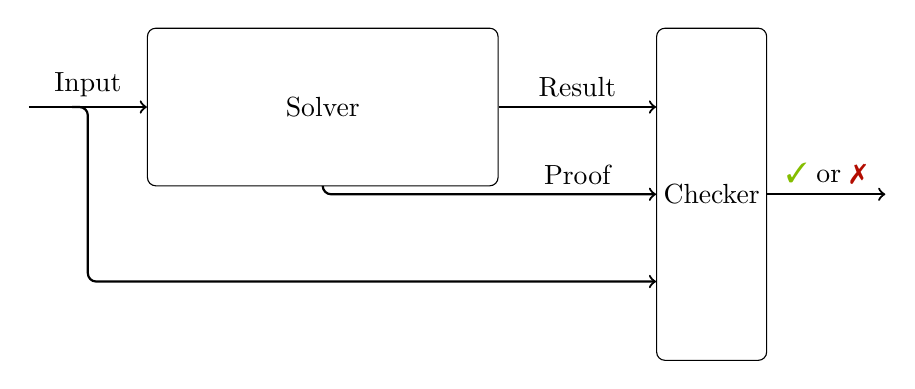
\begin{tikzpicture}
            \node (solver) [%
            inner xsep=5em,
            inner ysep=2.5em, 
            draw, rounded corners=3pt] { Solver };

            \node (checker) [%
            right=2cm of solver.north east, 
            anchor=north west,
            inner xsep=0.25em,
            draw, rounded corners=3pt, 
            minimum height=12em, 
            visible on=<3->] { Checker };

            \draw [->, thick] (solver.east) -- (solver.east -| checker.west)
                coordinate [midway] (solutionmid) node [above, midway]
                { 
                  Result
                };

            \draw [->, thick, rounded corners=3pt, visible on=<2->] (solver.south) -- (solver.south |- checker.west)
                -- (checker.west) coordinate [midway] (proofmid);

            \coordinate (prooflabel) at (proofmid-|solutionmid);
            \node [above=0cm of prooflabel, visible on=<2->] { Proof };

            \coordinate [right=1.5cm of checker.east] (verified);
            \draw [->, thick, visible on=<4->] (checker.east) -- (verified) node [above, midway] { \textcolor{uofglawn}{\ding{51}} or \textcolor{uofgpillarbox}{\ding{55}} };

            \coordinate [left=1.5cm of solver.west] (input);
            \draw [->, thick] (input) -- (solver.west) coordinate [midway] (inputmid) node [above, midway] { Input };

            \coordinate (checkerbotleft) at ($(checker.west)+($(checker.west)-(solver.east-|checker.west)$)$);

            \draw [->, thick, rounded corners=3pt, visible on=<3->] ($(inputmid)+(-0.2,0)$) -- (inputmid) -- (inputmid |- checkerbotleft) -- (checkerbotleft);
        \end{tikzpicture}
      \end{center}
    \vspace*{-0.7em}
  \begin{enumerate}
  \item<1->
    Run solver on problem input.
  \item<2->
    Get both a solution and a proof as output.
  \item<3->
    Feed input + solution + proof to proof checker.
  \item<4->
    Verify that proof checker says solution is correct.
  \end{enumerate}
\end{frame}

\begin{frame}{Pseudo-Boolean Problems}
    \begin{minipage}[t]{0.25\framewidth}
        \textcolor{uofgcobalt}{\textbf{Variables}}
    \end{minipage}\hfill\begin{minipage}[c]{0.70\framewidth}
        $x_i \in \{ 0, 1 \}$
    \end{minipage}\bigskip

    \begin{minipage}[t]{0.25\framewidth}
        \textcolor{uofgcobalt}{\textbf{Literals}}
    \end{minipage}\hfill\begin{minipage}[c]{0.70\framewidth}
        $\{ x_i, \overline{x}_i \}$

        \medskip

        $\overline{x}_i$ defined to be $1 - x_i$, means ``not $x$''
    \end{minipage}\bigskip

    \begin{minipage}[t]{0.25\framewidth}
        \textcolor{uofgcobalt}{\textbf{Constraints}}
    \end{minipage}\hfill\begin{minipage}[c]{0.70\framewidth}
        $\sum_i a_i x_i \bowtie A$ for $a_i, A \in \mathbb{Z}$ and $\bowtie \,\in \{ \le, \ge \}$

        \medskip
        Can rewrite into normalised form with $a_i, A \in \mathbb{N}$ and $\bowtie\,=\,\ge$
    \end{minipage}\bigskip

    \begin{minipage}[t]{0.25\framewidth}
        \textcolor{uofgcobalt}{\textbf{Objective}}
    \end{minipage}\hfill\begin{minipage}[c]{0.70\framewidth}
        Maximise $\sum_i a_i x_i$
    \end{minipage}\bigskip
\end{frame}

\begin{frame}{Knapsack as a Pseudo-Boolean Problem}
    \begin{align*}
        &2 x_1 + 5 x_2 + 2 x_3 + 3 x_4 + 2 x_5 + 3 x_6 \le 7 \\
        \text{maximise~} &2 x_1 + 4 x_2 + 2 x_3 + 5 x_4 + 4 x_5 + 3 x_6
    \end{align*}
\end{frame}

\begin{frame}{Implications as Pseudo-Boolean Constraints}
    Can express implications
    \begin{equation*} y \Rightarrow 3x_1 + 2x_2 + x_3 + x_4 \ge 3 \end{equation*}
    as
    \begin{equation*}
    3\overline{y} + 3x_1 + 2x_2 + x_3 + x_4 \ge 3
    \end{equation*}

    \bigskip

    We can also do $\land_i y_i \Rightarrow C$ and $y \Leftarrow C$.
\end{frame}

\begin{frame}{The VeriPB Proof System}
    \begin{center}
        \url{https://gitlab.com/MIAOresearch/software/VeriPB} \\
        \bigskip
    \end{center}
    \begin{itemize}
        \item MIT licence, written in Python with parsing in C++.
        \item Useful features like tracing and proof debugging.
    \end{itemize}
\end{frame}

\begin{frame}{Cutting Planes Proofs 1: Linear Inequalities}
    \begin{minipage}[c]{0.35\framewidth}
        \textcolor{uofgcobalt}{\textbf{Model axioms}}
    \end{minipage}\hfill\begin{minipage}[c]{0.60\framewidth}
        \centering From the input
    \end{minipage}\bigskip

    \begin{minipage}[c]{0.35\framewidth}
        \textcolor{uofgcobalt}{\textbf{Addition}}
    \end{minipage}\hfill\begin{minipage}[c]{0.60\framewidth}\begin{prooftree}
        \AxiomC{$\sum_i a_i \ell_i \ge A$}
        \AxiomC{$\sum_i b_i \ell_i \ge B$}
        \BinaryInfC{$\sum_i (a_i + b_i) \ell_i \ge A + B$}
    \end{prooftree}\end{minipage}\bigskip

    \begin{minipage}[c]{0.35\framewidth}
        \textcolor{uofgcobalt}{\textbf{Multiplication}}\\
        for any $c \in \mathbb{N^+}$
    \end{minipage}\hfill\begin{minipage}[c]{0.60\framewidth}\begin{prooftree}
        \AxiomC{$\sum_i a_i \ell_i \ge A$}
        \UnaryInfC{$\sum_i { c a_i \ell_i } \ge c A$}
    \end{prooftree}\end{minipage}
\end{frame}

\begin{frame}{Cutting Planes Proofs 2: 0-1 Variables}
    \begin{minipage}[c]{0.35\framewidth}
        \textcolor{uofgcobalt}{\textbf{Literal axioms}}
    \end{minipage}\hfill\begin{minipage}[c]{0.60\framewidth}\begin{prooftree}
        \AxiomC{~}
        \UnaryInfC{$\ell_i \ge 0$}
    \end{prooftree}\end{minipage}\bigskip

    \begin{minipage}[c]{0.35\framewidth}
        \textcolor{uofgcobalt}{\textbf{Division}}\\
        for any $c \in \mathbb{N^+}$
    \end{minipage}\hfill\begin{minipage}[c]{0.60\framewidth}\begin{prooftree}
        \AxiomC{$\sum_i a_i \ell_i \ge A$}
        \UnaryInfC{$\sum_i {\left\lceil \frac{a_i}{c} \right\rceil} \ell_i \ge \left\lceil \frac{A}{c} \right\rceil$}
    \end{prooftree}\end{minipage}\bigskip

    \begin{minipage}[c]{0.35\framewidth}
        \textcolor{uofgcobalt}{\textbf{Saturation}}
    \end{minipage}\hfill\begin{minipage}[c]{0.60\framewidth}\begin{prooftree}
        \AxiomC{$\sum_i a_i \ell_i \ge A$}
        \UnaryInfC{$\sum_i \operatorname{min}\left(a_i, A\right) \ell_i \ge A$}
    \end{prooftree}\end{minipage}
\end{frame}

\begin{frame}{CNF, Resolution, and Implications}
    Pseudo-Boolean constraints are a superset of CNF clauses:
    \begin{equation*}
        a \lor \overline{b} \lor c \qquad \Leftrightarrow \qquad a + \overline{b} + c \ge 1
    \end{equation*}

    CNF proofs can be done using the resolution rule:\bigskip

    \begin{minipage}[c]{0.35\framewidth}
        \textcolor{uofgcobalt}{\textbf{Resolution}}
    \end{minipage}\hfill\begin{minipage}[c]{0.60\framewidth}\begin{prooftree}
        \AxiomC{$a_1 \lor a_2 \lor \cdots \lor c$}
        \AxiomC{$\overline{c} \lor b_1 \lor b_2 \lor \cdots$}
        \BinaryInfC{$a_1 \lor a_2 \lor \cdots b_1 \lor b_2 \lor \cdots$}
    \end{prooftree}\end{minipage}\bigskip

    Another way of viewing this is:\bigskip

    \begin{minipage}[c]{0.35\framewidth}
        \textcolor{uofgcobalt}{\textbf{Resolution}}
    \end{minipage}\hfill\begin{minipage}[c]{0.60\framewidth}\begin{prooftree}
        \AxiomC{$(\overline{a}_1 \land \overline{a}_2 \land \cdots) \Rightarrow c$}
        \AxiomC{$c \Rightarrow (b_1 \lor b_2 \lor \cdots)$}
        \BinaryInfC{$(\overline{a}_1 \land \overline{a}_2 \land \cdots) \Rightarrow (b_1 \lor b_2 \lor \cdots)$}
    \end{prooftree}\end{minipage}\bigskip

    We can simulate this in cutting planes using addition then saturation.
\end{frame}

\begin{frame}{Extended Cutting Planes Proofs}
    We'll also need a way of introducing a new variable that are true if and only if a certain
    constraint holds (\emph{reification}).

    \bigskip

    \begin{minipage}[c]{0.35\framewidth}
        \textcolor{uofgcobalt}{\textbf{Extension}}\\
        $y$ a fresh variable \\
        $C$ any constraint
    \end{minipage}\hfill\begin{minipage}[c]{0.60\framewidth}\begin{prooftree}
        \AxiomC{~}
        \UnaryInfC{$y \Rightarrow C$ \qquad $y \Leftarrow C$}
    \end{prooftree}\end{minipage}

    \bigskip

    In reality: we have a more general extension rule, but we don't need it today.
\end{frame}

\begin{frame}{Unit Propagation for Clauses}

    \begin{align*}
        & a \lor \overline{b} \lor c \\
        & \overline{c} \lor d
    \end{align*}

    Suppose I tell you that $a$ must be false and $b$ must be true.

    \bigskip

    Must set $c$ to true to satisfy first clause.

    \bigskip

    Now must set $d$ to false to satisfy second clause.
\end{frame}

\begin{frame}{Unit Propagation for Constraints}
    \begin{align*}
        5a + 2b + 3c + d + e + f \ge 5
    \end{align*}

    Suppose I tell you that $a = 0$. Can't say anything yet.

    \bigskip

    Suppose I tell you that $b = 0$ as well. Then $c = 1$ must hold.

    \bigskip

    In general: integer bounds consistency. We can do this \emph{efficiently}.
\end{frame}

\begin{frame}{Reverse Unit Propagation}
    Let $C$ be any constraint. Suppose $\overline{C}$ unit propagates to contradiction. Then without
    loss of satisfaction, we can add $C$ as a new constraint.

    \bigskip

    \begin{minipage}[c]{0.35\framewidth}
        \textcolor{uofgcobalt}{\textbf{RUP}}\\
        $C$ any constraint
    \end{minipage}\hfill\begin{minipage}[c]{0.60\framewidth}\begin{prooftree}
        \AxiomC{$\overline{C}$ unit propagates to contradiction}
        \UnaryInfC{$C$}
    \end{prooftree}\end{minipage}

    \bigskip

    Can rewrite any RUP step as a sequence of cutting planes steps, but often writing RUP proofs is
    much more convenient.
\end{frame}

\begin{frame}{A Framework for Proofs for Backtracking Search}
\end{frame}

\begin{frame}{Proofs Under Implication}
    \begin{theorem}
    Let's say we have a collection of constraints $\mathcal{C}$ and know how to get a proof deriving
        $D$. \\\medskip

    Suppose now we replace one or more constraints $C_i$ from $\mathcal{C}$ with implications $\land
        G_i \Rightarrow C$. \\\medskip

    Then we know how to get a proof deriving $\land \cup_i G_i \Rightarrow D$.
    \end{theorem}
    \begin{proof}[Handwavy proof sketch]
        For RUP, add in the implications and it ``just works''. \\\medskip

        For cutting planes, run the same proof, but saturate between each step. Use literal
        axioms at the end to re-introduce any assumptions that disappear from $\land \cup_i G_i$,
        and to fix up coefficients. \\\medskip

        For extension rules, keep them as-is.
    \end{proof}
\end{frame}

\begin{frame}{Should You Trust the Checker?}
    \begin{center}
        \begin{tikzpicture}
            \node (solver) [ inner xsep=4em, inner ysep=2.5em, draw, rounded corners=3pt] { Solver };
            \node (elaborator) [ right=2cm of solver.north east, anchor=north west, inner
            xsep=0.25em, draw, rounded corners=3pt, minimum height=12em, text width=5em, text centered] {
                \only<1>{Checker}\only<2->{Elaborator} };
            \node (verifiedchecker) [ right=2cm of elaborator.north east, anchor=north west, inner
                xsep=0.25em, draw, rounded corners=3pt, minimum height=8em, text width=4em, text
                centered, yshift=-2cm, visible on=<3->] { Verified Checker };

            \draw [->, thick] (solver.east) -- (solver.east -| elaborator.west) coordinate [midway] (solutionmid) node [above, midway] { Result };

            \draw [->, thick, rounded corners=3pt] (solver.south) -- (solver.south |- elaborator.west) -- (elaborator.west) coordinate [midway] (proofmid);

            \coordinate (prooflabel) at (proofmid-|solutionmid); \node [above=0cm of prooflabel] { Proof };

            \coordinate [right=2cm of verifiedchecker.east] (verified);
            \draw [->, thick, visible on=<3->] (verifiedchecker.east) -- (verified)
                node [above, midway] { \textcolor{uofglawn}{\ding{51}} or \textcolor{uofgpillarbox}{\ding{55}} }
                node [below, midway, text centered, text width=5em] { Trusted Result };

            \coordinate [left=1.5cm of solver.west] (input);
            \draw [->, thick] (input) -- (solver.west) coordinate [midway] (inputmid) node [above, midway] { Input };

            \coordinate (verifiedcheckertopleft) at ($(verifiedchecker.west)+($(0cm,1.2cm)$)$);
            \draw [->, thick, visible on=<2->] (elaborator.east |- verifiedcheckertopleft) -- (verifiedcheckertopleft) node [above, midway, text width=4em, text centered] { Result };
            \draw [->, thick, visible on=<2->] (elaborator.east |- verifiedchecker.west) -- (verifiedchecker.west) node [above, midway, text width=4em, text centered] { Kernel Proof };

            \coordinate (elaboratorbotleft) at ($(elaborator.west)+($(elaborator.west)-(solver.east-|elaborator.west)$)$);
            \coordinate (verifiedcheckerbotleft) at ($(verifiedchecker.west)+($(0cm,-1.2cm)$)$);

            \draw [->, thick, rounded corners=3pt] ($(inputmid)+(-0.2,0)$) -- (inputmid) -- (inputmid |- elaboratorbotleft) -- (elaboratorbotleft);
            \draw [->, thick, rounded corners=3pt, visible on=<3->] ($(inputmid)+(-0.2,0)$) -- (inputmid) -- (inputmid |- verifiedcheckerbotleft) -- (verifiedcheckerbotleft);

            \coordinate (elaboratortopright) at ($(elaborator.east)+($(verifiedcheckertopleft)-(verifiedchecker.west)$)$);
            \draw [->, thick] (elaboratortopright) -- (elaboratortopright-|verifiedchecker.west)
                node [above, midway] { \textcolor{uofglawn}{\ding{51}} or \textcolor{uofgpillarbox}{\ding{55}} };
        \end{tikzpicture}
      \end{center}
\end{frame}

\section{Proofs for Knapsack}

\begin{frame}{Proofs for Dynamic Programming Algorithms for Knapsack}
\end{frame}

\begin{frame}{Extension Variables for States}
    For each state (or entry in the matrix) on layer $\ell$, create extension variables
    \begin{align*}
        W^{\ell}_{w} &\Leftrightarrow \sum_{i=1}^{\ell} \boldsymbol{w}_i x_i \ge w \\
        P^{\ell}_{p} &\Leftrightarrow \sum_{i=1}^{\ell} \boldsymbol{p}_i x_i \le p \\
        N^{\ell}_{w,p} & \Leftrightarrow W^{\ell}_{w} + P^{\ell}_{p} \ge 2
    \end{align*}
\end{frame}

\begin{frame}[t]{Transitioning Between States}
    \begin{minipage}[t]{0.3\framewidth}
    \uncover<1->{
        We don't have to take an item on layer $\ell$, so need to prove:
        \begin{align*}
            W^{\ell-1}_{w} \land \overline{x}_\ell &\Rightarrow W^\ell_\mathit{w} \\
            P^{\ell-1}_{p} \land \overline{x}_\ell &\Rightarrow P^\ell_\mathit{p} \\
            N^{\ell-1}_{w,p} \land \overline{x}_\ell &\Rightarrow N^\ell_{w,p}
        \end{align*}
    }
    \end{minipage}\hfill\begin{minipage}[t]{0.30\framewidth}
    \uncover<2->{
        If we can't take item on layer $\ell$, need to prove:
        \begin{align*}
            W^{\ell-1}_{w} &\Rightarrow \overline{x}_\ell \\
            N^{\ell-1}_{w,p} &\Rightarrow \overline{x}_\ell  \\
            N^{\ell-1}_{w,p} &\Rightarrow N^\ell_{w,p}
        \end{align*}
    }
    \end{minipage}\hfill\begin{minipage}[t]{0.35\framewidth}
    \uncover<3->{
        If we can take item on layer $\ell$, we need to prove:
        \begin{align*}
            W^{\ell-1}_{w} \land x_\ell &\Rightarrow W^\ell_{w'} \\
            P^{\ell-1}_{p} \land x_\ell &\Rightarrow P^\ell_{p'} \\
            N^{\ell-1}_{w,p} \land x_\ell &\Rightarrow N^\ell_{w',p'} \\
            N^{\ell-1}_{w,p} &\Rightarrow N^\ell_{w,p} + N^\ell_{w',p'} \ge 1
        \end{align*}
        where
        \begin{align*}
            (w', p') &= (w + \boldsymbol{w}_\ell, p + \boldsymbol{p}_\ell)
        \end{align*}
    }
    \end{minipage}
\end{frame}

\begin{frame}{Merged States}
    For each $N^\ell_{w,p}$ that is dominated by some other $N^\ell_{w',p'}$, we prove
        $N^\ell_{w,p} \Rightarrow N^\ell_{w',p'}$.

        \medskip

    We can do this by unwrapping the conjunction, proving
    \begin{align*}
        & W^\ell_{w} \Rightarrow W^\ell_{w'} & \text{i.e.} && (\sum_{i=1}^{\ell} \boldsymbol{w}_i
        x_i \ge w) \Rightarrow (\sum_{i=1}^{\ell} \boldsymbol{w}_i x_i \ge w') &\text{~for some~} w' \le w \\
        & P^\ell_{p} \Rightarrow P^\ell_{p'} & \text{i.e.} && (\sum_{i=1}^{\ell} \boldsymbol{p}_i
        x_i \ge p) \Rightarrow (\sum_{i=1}^{\ell} \boldsymbol{p}_i x_i \ge p') &\text{~for some~} p' \ge p \\
    \end{align*}
    ``If there is an assignment to the first $\ell$ $x_i$ variables where the weight sums to at
    least 7 and the profit to no more than 4, then there is an assignment where the weight sums
    to at least 6 and the profit to no more than 5''.
\end{frame}

\begin{frame}{Establishing Completeness}
    Must show that we have to be in one of the states on this layer,
    \begin{align*}
        \sum_{(w,p)~\text{on layer}~\ell} N^\ell_{w,p} \ge 1
    \end{align*}

    We can use the at-least-one constraint
    \begin{align*}
        \sum_{(w,p)~\text{on layer}~\ell - 1} N^{\ell-1}_{w,p} \ge 1
    \end{align*}
    from the previous layer, and resolve on each \begin{align*}
        N^{\ell-1}_{w,p} &\Rightarrow N^\ell_{w,p} + N^\ell_{w',p'} \ge 1 &&\text{or}&
        N^{\ell-1}_{w,p} &\Rightarrow N^\ell_{w,p}
    \end{align*}
\end{frame}

\begin{frame}{Reading Off a Conclusion}
\end{frame}

\section{Knapsack Constraints}

\begin{frame}{Knapsack as a Constraint}
    \begin{align*}
        &x_i \in \{0, 1, \text{maybe other non-negative values}\}\\
        &W, P \in \{\text{some domain of non-negative values}\}\\
        &W = \sum_i \boldsymbol{w}_i x_i\\
        &P = \sum_i \boldsymbol{p}_i x_i
    \end{align*}

    Now we can have lower and upper bounds on both $W$ and $P$, and maybe we can reason that some
    items must or must not be taken.

    \medskip

    Effectively we're solving two (or one, or more?) non-negative integer linear equations simultaneously.
\end{frame}

\begin{frame}{A Change of States}
    For each state (or entry in the matrix) on layer $\ell$, define
    \begin{align*}
        W{\uparrow}^{\ell}_{w} &\Leftrightarrow \sum_{i=1}^{\ell} \boldsymbol{w}_i x_i \ge w
        &&\text{and}&
        W{\downarrow}^{\ell}_{w} &\Leftrightarrow \sum_{i=1}^{\ell} \boldsymbol{w}_i x_i \le w \\
        P{\uparrow}^{\ell}_{p} &\Leftrightarrow \sum_{i=1}^{\ell} \boldsymbol{p}_i x_i \ge p
        &&\text{and}&
        P{\downarrow}^{\ell}_{p} &\Leftrightarrow \sum_{i=1}^{\ell} \boldsymbol{p}_i x_i \le p
    \end{align*}\begin{align*}
        N^{\ell}_{w,p} & \Leftrightarrow W{\uparrow}^{\ell}_{w} + W{\downarrow}^{\ell}_{w} + P{\uparrow}^{\ell}_{p} + P{\downarrow}^{\ell}_{p} \ge 4
    \end{align*}
    So now our states represent \emph{exact} weights and profits.
\end{frame}

\begin{frame}{A Change of Merge Rules}
    We can still use the maximum rule to merge \begin{equation*}
        \sum_{i=1}^{\ell} \boldsymbol{w}_i = w \text{~and~} \sum_{i=1}^{\ell} \boldsymbol{p}_i = p
        \qquad \text{or} \qquad
        \sum_{i=1}^{\ell} \boldsymbol{w}_i = w \text{~and~} \sum_{i=1}^{\ell} \boldsymbol{p}_i = p'
    \end{equation*}
    with $p > p'$.

    \bigskip

    We can no longer merge states where
    \begin{equation*}
            \sum_{i=1}^{\ell} \boldsymbol{w}_i = w \text{~and~} \sum_{i=1}^{\ell} \boldsymbol{p}_i = p
            \qquad \text{or} \qquad
            \sum_{i=1}^{\ell} \boldsymbol{w}_i = w' \text{~and~} \sum_{i=1}^{\ell} \boldsymbol{p}_i = p'
    \end{equation*}
    with $p \ge p'$ and $w \le w'$.

    \bigskip

    Reassuringly, the proofs won't work if you try this\ldots

\end{frame}

\begin{frame}{Establishing Arc Consistency}
    We can read off all possible values for $P$ and $W$ from the final layer.

    \bigskip

    Easy to use this and resolution with the at-least-one constraint to eliminate all
    other values.

    \bigskip

    But what about the $x_i$ variables?
\end{frame}

\begin{nearlyplainframe}[t]{Forced and Forbidden Items}
\tikzstyle{level 1}=[level distance=2.20cm, sibling distance=4.00cm]
\tikzstyle{level 2}=[level distance=2.20cm, sibling distance=2.00cm]
\tikzstyle{level 3}=[level distance=2.20cm, sibling distance=1.00cm]
\tikzstyle{level 4}=[level distance=2.20cm, sibling distance=0.75cm]
\tikzstyle{level 5}=[level distance=2.20cm, sibling distance=0.50cm]
\tikzstyle{level 6}=[level distance=2.20cm, sibling distance=0.30cm]
\vspace*{-1cm}
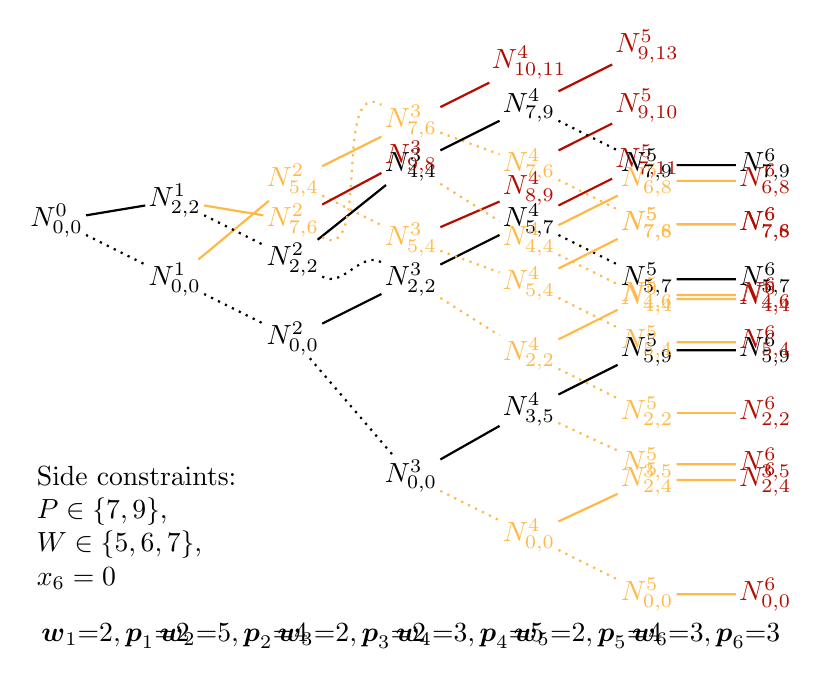
\begin{tikzpicture}[grow=right, sloped]
    \node (N0w0p0) [state] {$N^0_{0,0}$}
    child {
        node (N1w0p0) [state] {$N^1_{0,0}$}
        child {
            node (N2w0p0) [state] {$N^2_{0,0}$}
            child {
                node (N3w0p0) [state, yshift=-1.0cm] {$N^3_{0,0}$}
                child {
                    node (N4w0p0) [state, backwards] {$N^4_{0,0}$}
                    child {
                        node (N5w0p0) [state, backwards] {$N^5_{0,0}$}
                        child {
                            node (N6w0p0) [state, infeasible] {$N^6_{0,0}$}
                            edge from parent [accept, backwards]
                        }
                        edge from parent [reject, backwards]
                    }
                    child {
                        node [state, backwards, yshift=-0.05cm] {$N^5_{2,4}$}
                        child {
                            node [state, infeasible] {$N^6_{2,4}$}
                            edge from parent [accept, backwards]
                        }
                        edge from parent [accept, backwards]
                    }
                    edge from parent [reject, backwards]
                }
                child {
                    node [state, yshift=0.1cm] {$N^4_{3,5}$}
                    child {
                        node [state, backwards, yshift=0.05cm] {$N^5_{3,5}$}
                        child {
                            node [state, infeasible] {$N^6_{3,5}$}
                            edge from parent [accept, backwards]
                        }
                        edge from parent [reject, backwards]
                    }
                    child {
                        node [state] {$N^5_{5,9}$}
                        child {
                            node [state] {$N^6_{5,9}$}
                            edge from parent [accept]
                        }
                        edge from parent [accept]
                    }
                    edge from parent [accept]
                }
                edge from parent [reject]
            }
            child {
                node (N3w2p2) [state] {$N^3_{2,2}$}
                child {
                    node [state, backwards, yshift=-0.2cm] {$N^4_{2,2}$}
                    child {
                        node [state, backwards] {$N^5_{2,2}$}
                        child {
                            node [state, infeasible] {$N^6_{2,2}$}
                            edge from parent [accept, backwards]
                        }
                        edge from parent [reject, backwards]
                    }
                    child {
                        node [state, backwards] {$N^5_{4,6}$}
                        child {
                            node [state, infeasible] {$N^6_{4,6}$}
                            edge from parent [accept, backwards]
                        }
                        edge from parent [accept, backwards]
                    }
                    edge from parent [reject, backwards]
                }
                child {
                    node [state] {$N^4_{5,7}$}
                    child {
                        node [state] {$N^5_{5,7}$}
                        child {
                            node [state] {$N^6_{5,7}$}
                            edge from parent [accept]
                        }
                        edge from parent [reject]
                    }
                    child {
                        node [state, infeasible] {$N^5_{7,11}$}
                        edge from parent [accept, infeasible]
                    }
                    edge from parent [accept]
                }
                edge from parent [accept]
            }
            edge from parent [reject]
        }
        child {
            node (N2w5p5) [state, backwards, yshift=0.5cm] {$N^2_{5,4}$}
            child {
                node [state, backwards] {$N^3_{5,4}$}
                child {
                    node [state, backwards, yshift=0.2cm] {$N^4_{5,4}$}
                    child {
                        node [state, backwards] {$N^5_{5,4}$}
                        child {
                            node [state, infeasible] {$N^6_{5,4}$}
                            edge from parent [accept, backwards]
                        }
                        edge from parent [reject, backwards]
                    }
                    child {
                        node [state, backwards] {$N^5_{7,8}$}
                        child {
                            node [state, infeasible] {$N^6_{7,8}$}
                            edge from parent [accept, backwards]
                        }
                        edge from parent [accept, backwards]
                    }
                    edge from parent [reject, backwards]
                }
                child {
                    node [state, infeasible, yshift=-0.1cm] {$N^4_{8,9}$}
                    edge from parent [accept, infeasible]
                }
                edge from parent [reject, backwards]
            }
            child {
                node (N3w7p6) [state, backwards] {$N^3_{7,6}$}
                child {
                    node [state, backwards, yshift=0.2cm] {$N^4_{7,6}$}
                    child {
                        node [state, backwards] {$N^5_{7,6}$}
                        child {
                            node [state, infeasible] {$N^6_{7,6}$}
                            edge from parent [accept, backwards]
                        }
                        edge from parent [reject, backwards]
                    }
                    child {
                        node [state, infeasible] {$N^5_{9,10}$}
                        edge from parent [accept, infeasible]
                    }
                    edge from parent [reject, backwards]
                }
                child {
                    node [state, infeasible] {$N^4_{10,11}$}
                    edge from parent [accept, infeasible]
                }
                edge from parent [accept, backwards]
            }
            edge from parent [accept, backwards]
        }
        edge from parent [reject]
    }
    child {
        node [state, yshift=-0.5cm] {$N^1_{2,2}$}
        child {
            node (N2w2p2) [state] {$N^2_{2,2}$}
            child {
                node [state, yshift=1.2cm] {$N^3_{4,4}$}
                child {
                    node [state, backwards, yshift=-0.2cm] {$N^4_{4,4}$}
                    child {
                        node [state, backwards] {$N^5_{4,4}$}
                        child {
                            node [state, infeasible] {$N^6_{4,4}$}
                            edge from parent [accept, backwards]
                        }
                        edge from parent [reject, backwards]
                    }
                    child {
                        node [state, backwards] {$N^5_{6,8}$}
                        child {
                            node [state, infeasible] {$N^6_{6,8}$}
                            edge from parent [accept, backwards]
                        }
                        edge from parent [accept]
                    }
                    edge from parent [reject, backwards]
                }
                child {
                    node [state] {$N^4_{7,9}$}
                    child {
                        node [state] {$N^5_{7,9}$}
                        child {
                            node [state] {$N^6_{7,9}$}
                            edge from parent [accept]
                        }
                        edge from parent [reject]
                    }
                    child {
                        node [state, infeasible] {$N^5_{9,13}$}
                        edge from parent [accept, infeasible]
                    }
                    edge from parent [accept]
                }
                edge from parent [accept]
            }
            edge from parent [reject]
        }
        child {
            node (N2w7p6) [state, backwards, yshift=-1cm] {$N^2_{7,6}$}
            child {
                node [state, infeasible, yshift=0.8cm] {$N^3_{9,8}$}
                edge from parent [accept, infeasible]
            }
            edge from parent [accept, backwards]
        }
        edge from parent [accept]
    };

    \draw [reject, out=330, in=150] (N2w2p2) to (N3w2p2);
    \draw [reject, backwards, out=330, in=150] (N2w7p6) to (N3w7p6);

    \coordinate (B1x) at ($(N0w0p0)!0.5!(N1w0p0)$);
    \coordinate (B1) at (B1x|-N6w0p0);
    \node [below=0.25cm of B1] {$\boldsymbol{w}_1{=}2, \boldsymbol{p}_1{=}2$};

    \coordinate (B2x) at ($(N1w0p0)!0.5!(N2w0p0)$);
    \coordinate (B2) at (B2x|-N6w0p0);
    \node [below=0.25cm of B2] {$\boldsymbol{w}_2{=}5, \boldsymbol{p}_2{=}4$};

    \coordinate (B3x) at ($(N2w0p0)!0.5!(N3w0p0)$);
    \coordinate (B3) at (B3x|-N6w0p0);
    \node [below=0.25cm of B3] {$\boldsymbol{w}_3{=}2, \boldsymbol{p}_3{=}2$};

    \coordinate (B4x) at ($(N3w0p0)!0.5!(N4w0p0)$);
    \coordinate (B4) at (B4x|-N6w0p0);
    \node [below=0.25cm of B4] {$\boldsymbol{w}_4{=}3, \boldsymbol{p}_4{=}5$};

    \coordinate (B5x) at ($(N4w0p0)!0.5!(N5w0p0)$);
    \coordinate (B5) at (B5x|-N6w0p0);
    \node [below=0.25cm of B5] {$\boldsymbol{w}_5{=}2, \boldsymbol{p}_5{=}4$};

    \coordinate (B6x) at ($(N5w0p0)!0.5!(N6w0p0)$);
    \coordinate (B6) at (B6x|-N6w0p0);
    \node [below=0.25cm of B6] {$\boldsymbol{w}_6{=}3, \boldsymbol{p}_6{=}3$};

    \coordinate (SC) at ($(N0w0p0.west)+(0cm,-3cm)$);
    \node [anchor=north west, text width=8em] at (SC) {Side constraints:
    \\$P \in \{7, 9\}$,
    \\$W \in \{5, 6, 7\}$,
    \\$x_6 = 0$};
\end{tikzpicture}
\end{nearlyplainframe}

\begin{frame}{It Works}
\end{frame}

\begin{frame}{So What?}
    \begin{itemize}
        \item This is a general framework, not specific to knapsack.
        \item We can do dynamic programming / decision diagram propagators for CP.
        \item All of this is in a unified proof setting.
            \begin{itemize}
                \item In particular, nothing in the proof system knows about ``search'' or
                    ``states''.
                \item We can reason about complex states using the full power of cutting
                    planes.
                \item We could do symmetry reasoning (two identical items) and dominance reasoning
                    (one item better than another) too.
            \end{itemize}
        \item Key proof technique is that we can wrap and unwrap extension variables and implications.
        \item Might help us start to trust some of these clever hybrid algorithms
            for graph parameters like treewidth?
    \end{itemize}
\end{frame}

{
    \usebackgroundtemplate{
        \tikz[overlay, remember picture]
        \node[at=(current page.south), anchor=south, yshift=-1cm, inner sep=0pt]{\includegraphics[keepaspectratio=true, width=\paperwidth]{../../images/background2.jpg}};
    }

    \begin{frame}[plain,noframenumbering]
        \begin{tikzpicture}[remember picture, overlay]
            \node at (current page.north west) {
                \begin{tikzpicture}[remember picture, overlay]
                    \fill [fill=uofguniversityblue, anchor=north west] (0, 0) rectangle (\paperwidth, -2.8cm);
                \end{tikzpicture}
            };

            \node (logo) [anchor=north east, shift={(-0.8cm,-0.2cm)}] at (current page.north east) {
                
\includegraphics[keepaspectratio=true,scale=0.5]{../../images/UoG_keyline.pdf}
            };

            \node (logo2) [anchor=north, below=0.2cm of logo.south] {
                
\includegraphics[keepaspectratio=true,scale=0.1]{../../images/RAEngWhite.pdf}
            };

            \coordinate (logos) at ($(logo.south)!0.5!(logo2.north)$);

            \node [anchor=west, xshift=0.8cm] at (current page.west |- logos) {
                \begin{minipage}{0.60\paperwidth}\raggedright
                    \textcolor{white}{\url{https://ciaranm.github.io/}} \\[0.3cm]
                    \textcolor{white}{\href{mailto:ciaran.mccreesh@glasgow.ac.uk}{\nolinkurl{ciaran.mccreesh@glasgow.ac.uk}}}
                \end{minipage}
            };
        \end{tikzpicture}
    \end{frame}
}

\end{document}

